\typeout{comp551 writeup template}

% These are the instructions for authors for IJCAI-19.

\documentclass[11pt]{article}
\pdfpagewidth=8.5in
\pdfpageheight=11in
\usepackage{comp551}

% Use the postscript times font!
%\usepackage{times}
\usepackage{tabu}
\usepackage{pgfplots}
\usepackage{graphicx}
\usepackage{soul}
\usepackage{url}
\usepackage[hidelinks]{hyperref}
\usepackage[utf8]{inputenc}
\usepackage[small]{caption}
\usepackage{graphicx}
\usepackage{amsmath}
\usepackage{booktabs}
\urlstyle{same}

% the following package is optional:
\usepackage{latexsym} 

\title{MiniProject 1: Predicting the Popularity of Reddit Comments using Linear Regression}

\author{%
\begin{tabular}{c} Jean-Sébastien Grondin \\ \normalfont McGill Id:260345519  \\ \normalfont \small jean-sebastien.grondin@mail.mcgill.ca \end{tabular} 
\begin{tabular}{c} Zhourong Li \\ \normalfont McGill Id:260674414  \\ \normalfont \small zhourong.li@mail.mcgill.ca \end{tabular} 
\begin{tabular}{c} Zhenze Han \\ \normalfont McGill Id:260675404  \\ \normalfont \small zhenze.han@mail.mcgill.ca \end{tabular} }

\begin{document}

\maketitle

\begin{abstract}
This paper presents the methodology and results obtained when using linear regression to predict the popularity of Reddit comments. This study used a dataset of 12000 instances which was split into training, validation and test sets. Available features included text comments, the number of replies comments received (i.e. $children$), an indication of whether each comment was the root of a thread and an indicator of controversiality.  Several additional features were extracted and analyzed for improving the model performance. The mean squared error (MSE) was used to compare models and assess the performance. We confirmed that the closed form solution was most effective (faster, more robust and the exact solution). The model complexity was incrementally increased to find the optimal error on the validation set. The following features were added to the final model: a 60-dimensional feature vector $x_{counts}$ corresponding to the 60 most frequently occuring words in the training set, the number of $children^{2}$ and an interaction feature for the controversiality times the natural log of the children. The final model achieved a MSE of  \textbf{X.XXX} on the test set. 
\end{abstract}

\section{Introduction}
Reddit is a popular social media site which is currently the 5th most popular website in the United States according to Alexa. It is essentially a massive collection of forums and threads where users can upvote or downvote comments that they like or dislike (see an example below). Predicting reddit posts popularity was attempted in recent years \cite{thesis}\cite{stanford}\cite{TowardsDS} and has been found to be amenable to machine learning. \\
\\
\includegraphics[width=8cm]{reddit}\\
\\
The objective of this study was to implement and evaluate a linear regression model for predicting the popularity score of Reddit comments. A total of 12000 instances of text comments were used, in addition to other features such as the controversiality score and the number of replies each comment received. Text comments were processed in order to extract a word count occurence feature for the most frequently occuring words. Several other features were generated, and the two features which exhibited the highest correlation with the popularity score were retained. Both the closed form and the gradient descent solutions were implemented and compared. The mean squared error (MSE) was the metric used for all comparisons and analysis. The closed-form approach was used for subsequent experiments as it was found to be faster and more stable and also because it yields the exact solution. Models which included word occurence features for the 160 most frequent words in the training set were found to overfit compared to models that did not include as many words. It was found that only using the top 60 words prevented the overfit. The two new features that were extracted were shown to improve the model performance without causing overfitting. The final model achieved a mean squared error of \textbf{X.XXX} on the test set. 


\section{Dataset}

The original dataset was obtained from the subreddit community \textbf{r/Askreddit}. The dataset contained 12000 instances  with the following information:

\begin{itemize}
    	\item \textbf{popularity\_score:} This metric indicates how popular each comment is and is computed by Reddit. This is the target variable in this study. 
   	\item \textbf{children:} This feature indicates how many replies each comment received.
    	\item \textbf{is\_root:} This feature is True when a comment is the "root" of a conversation and is False when it is a reply to another comment.
    	\item \textbf{controversiality:} This feature is a binary variable that indicates if a comment is controversial (when equals 1) or not controversial (when equals 0). A controversial comment is one that receives close to the same amount of upvotes and downvotes.
    	\item \textbf{text:} The raw text of each comment.
\end{itemize}

The is\_root boolean values were encoded using 0 and 1.  The dataset was then split into training (80\%), validation (10\%) and test (10\%) sets and the training set was subsequently used for text processing, exploratory data analysis and feature extraction. Simple pre-processing was applied to text comments by first a) lower-casing all text and then b) spliting text based on whitespace tokens to generate a list of all words. A list of the 160 most frequently occurring words in the training data was then computed. For every text comments, a 160-dimensional feature vector, $x_{counts}$, was extracted, with $x_{counts}[i]$ being equal to the number of times the ith most frequent word occured in the comment. Using the same list, word occurence feature vectors were extracted for the test and validation sets. 
\\

Some exploratory data analysis was also achieved. The following figure gives a visual representation of the original non-text features. Several observations were made. The popularity score was found to increase with an increasing number of children. Also, controversial comments generally did not lead to high popularity nor high number of children. While it is not readily noticeable in the plot, the mean popularity score is slightly higher (0.981) for non-root comments compared to root comments (0.703), and the [min, max] range is also shorter [-6.267, 7.981] for non-root comments than for root comments [-6.779, 8.373]. \\
\\
\includegraphics[width=8.5cm, height=6cm]{EDA-1}\\
\\
Since children seemed to be somewhat correlated with the popularity, the following additional features were generated for further analysis: $children^{2}$, $children^{3}$, $ \ln children$, $(\ln children)*(1-controversiality)$. Also, two additional features were also extracted from the text comments: a) the length of each comment and b) the number of exclamation marks occurring in each comment. A correlation matrix heatmap was then computed to assess the correlation of features with the target variable and is displayed below: \\
\\
\includegraphics[width=8.5cm, height=6cm]{EDA-4}\\
\\
The two additional text related features mentioned above were not investigated further as they did not seem to be sufficiently correlated to the target variable. As for the others, a discussion of how these contribute to the model performance is included in the following section.\\
\\
Before moving on to the results section, readers should be wary of the ethical implications of using machine learning with social media data for analyzing or filtering information. Machine learning models can introduce several types of bias related to the way data is collected, models are built, etc. If these models are used to provide intelligence, or to make decisions on what information is important (e.g. what to read? what to watch? what to buy?), then this could have drastic societal consequences.  Readers should be cautious not to misuse these models or misinterpret the results, especially if they are deployed to the mass.\\

\section{Results}

Following are the results from comparing the training runtime speed when computing the closed-form solution and running the gradient descent algorithm. One should note that the records were based on the performance of an intel i9 processor, thus the runtime may vary when using different machines.  For these experiments, the text features were safely ignored and only the three features provided in the original dataset were used. Also, the hyper-parameters used were $eta_0$ = 0.000006, $beta$ = 0, $eps$ = 0.0001. For information, the MSE is also reported for the training set and the validation set. Although the gradient descent approach has essentially the same performance in terms of MSE in the following table, it does require more efforts and time for fine-tuning the hyper-parameters and achieve the same performance. The closed-form solution is obtained more rapidly without the need for fine-tuning hyperparameters and is also the exact solution.  It was also found that the validation MSE is lower than the training MSE, which is a consequence of how the data was split. Getting more data overall could help us mitigate this effect. \\

\begin{table}[h]
\centering
\begin{small}
\begin{tabular}[c]{|c|c|c|c|}
  \hline
   & Runtime & Training & Validation \\
   & (ms) & MSE & MSE \\
   \hline
  Closed Form & 128.29 & 1.08468 & 1.02033\\
  Gradient Descent & 231.91 & 1.08474 & 1.02067\\
  \hline
\end{tabular}
\end{small}
\end{table}

One should note that the accuracy of the closed-form solution is sensitive to its hyperparameters. For example, the Figure below shows the sensitivity of the training MSE on the hyperparameter $beta$, for $eta_0$ = 0.000006 and $eps$ = 0.0001. It is found that for a well tuned $beta$, it is possible to improve the training and validation MSE. This is because the alpha becomes smaller and smaller over the iterations which allows getting closer to the exact solution. However, when the $beta$ is set too high, after a certain number of iterations, the gradient step becomes so small that the convergence criterion (based on  $||w_{i} - w_{i-1}||_{2}$) is met even though the lowest error is not achieved. Given that the gradient descent solution converges very quickly, it was found that it is more convenient to set $beta$ to 0 and only adjust the other two hyperparameters: $eta_0$, and $eps$.\\ 
\\
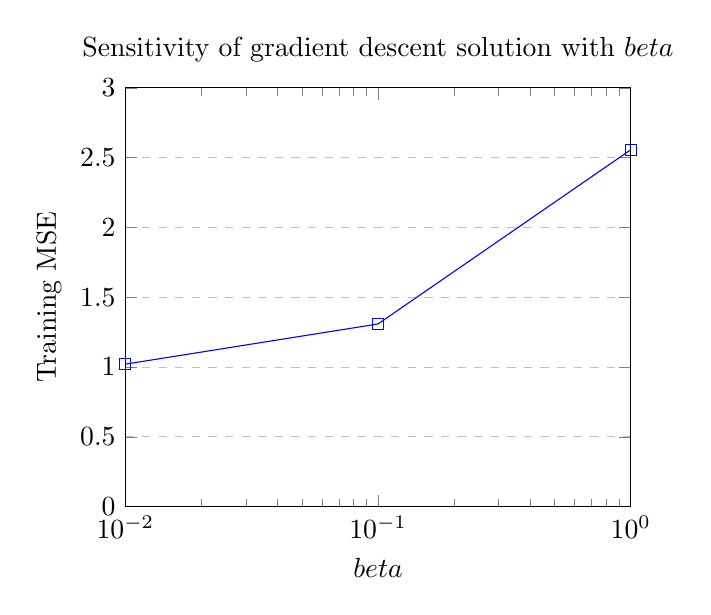
\begin{tikzpicture}
\begin{semilogxaxis}[
    title={Sensitivity of gradient descent solution with $beta$},
    xlabel={$beta$},
    ylabel={Training MSE},
    width=8cm,
    xmin=1e-2, xmax=1,
    ymin=0, ymax=3,
    xtick={1e-2, 1e-1, 1},
    ytick={0,0.5,1,1.5,2,2.5,3},
    ymajorgrids=true,
    grid style=dashed,
    ] 
   \addplot[
    color=blue,
    mark=square,
    ]
    coordinates {
    (1e-2,1.02067)(1e-1,1.30868)(1,2.55653)
    }; 
\end{semilogxaxis}
\end{tikzpicture}

The following figure shows the sensitivity of the training MSE when we fix $beta = 0$ and $eps = 0.0001$ and change the $eta_0$ value. It is found that with an increasing $eta_0$, the training MSE decreases, which goes against the intuition. It is known that although a larger $eta_0$ will yield faster runtimes (if convergence is achieved), it is likely not to achieve a smaller MSE than with a smaller $eta_0$ values. However, in this case this indicates that the $eps$ may be set too high in relation to the $eta_0$, which means the convergence criterion is met even though we could continue on the gradient descent and achieve a lower MSE had we set the $eps$ to a lower value.\\ 
\\ 
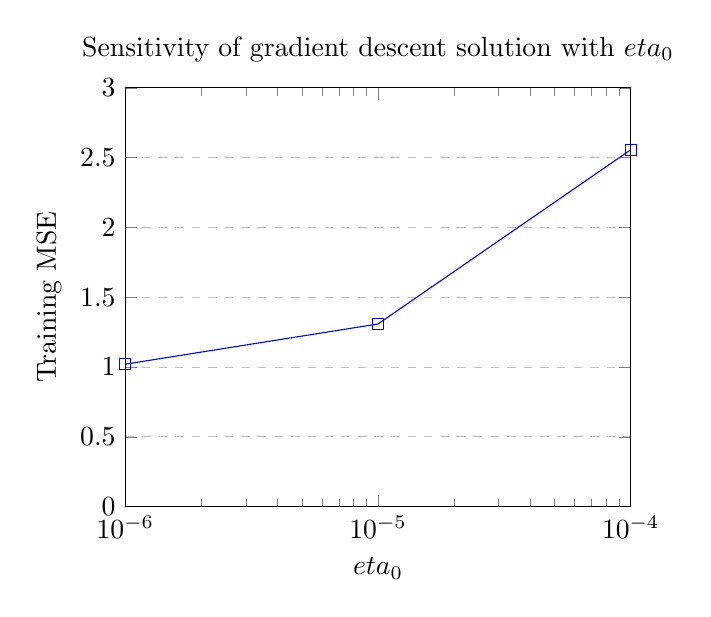
\begin{tikzpicture}
\begin{semilogxaxis}[
    title={Sensitivity of gradient descent solution with $eta_0$},
    xlabel={$eta_0$},
    ylabel={Training MSE},
    width=8cm,
    xmin=1e-6, xmax=1e-4,
    ymin=0, ymax=3,
    xtick={1e-6, 1e-5, 1e-4},
    ytick={0,0.5,1,1.5,2,2.5,3},
    ymajorgrids=true,
    grid style=dashed,
    ] 
   \addplot[
    color=blue,
    mark=square,
    ]
    coordinates {
    (1e-6,1.02067)(1e-5,1.30868)(1e-4,2.55653)
    }; 
\end{semilogxaxis}
\end{tikzpicture}

The next Figure shows the impact of fixing $eta_0 = 4e-05$ and $beta$ = 0 and computing the training set MSE with changing $eps$ values. This figure confirms the intuition. Lowerering the $eps$ brings the training MSE closer to the exact solution MSE but the incremental improvements are getting smaller and smaller. One should note that if the $eps$ is set too small, convergence may not be achieved. In summary, finding the optimal hyperparameters can be a challenging and iterative process. Hence, it was then decided that for the subsequent analysis, the closed-form approach would be used since it is faster, more robust but also yields the exact solution. \\ 
\\
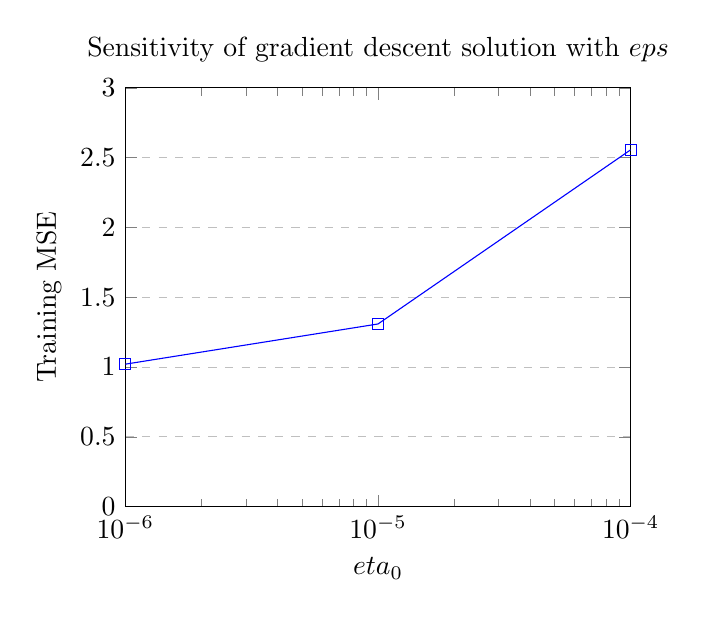
\begin{tikzpicture}
\begin{semilogxaxis}[
    title={Sensitivity of gradient descent solution with $eps$},
    xlabel={$eta_0$},
    ylabel={Training MSE},
    width=8cm,
    xmin=1e-6, xmax=1e-4,
    ymin=0, ymax=3,
    xtick={1e-6, 1e-5, 1e-4},
    ytick={0,0.5,1,1.5,2,2.5,3},
    ymajorgrids=true,
    grid style=dashed,
    ] 
   \addplot[
    color=blue,
    mark=square,
    ]
    coordinates {
    (1e-6,1.02067)(1e-5,1.30868)(1e-4,2.55653)
    }; 
\end{semilogxaxis}
\end{tikzpicture}

Three different linear regression models were trained to identify a reasonable number of the most frequent words to use in the features: one without text features, one which used the top 60 most frequent words and one which used the whole 160 list. The results are summarized in the next table. It is found that the model with 163 features (i.e. 160 word features + 3 non-text original features) is over fitting while the model with only the original 3 features is under fitting. The validation MSE is optimal when only using the top 60 words.\\ 
\\

\begin{table}[h]
\centering
\begin{small}
\begin{tabular}[c]{|c|c|c|c|}
  \hline
   & no text & top 60 & top 160 \\
   & feature & words & words \\
   \hline
  Training set MSE & 1.0847 & 1.0604 & 1.0478\\
  Validation set MSE & 1.0203 & 0.9839 & 0.9951\\
  \hline
\end{tabular}
\end{small}
\end{table}

Then we have incrementally added the new features that were extracted, starting with the most promising ones: $children^{2}$ and $(\ln children)*(1-controversiality)$. The results are shown in the next table. The trend is the same no matter how many of the most frequent words are added. Adding in the $children^{3}$ was found to lead to overfitting the model and thus was dropped. Hence, the final model chosen for predicting the popularity score in the test set had the following features: a 60-dimensional feature vector $x_{counts}$ corresponding to the 60 most frequently occuring words in the training set, $is\_root$, $controversiality$, $children$, $children^{2}$ and $(\ln children)*(1-controversiality)$. A MSE of \textbf{X.XXX} was obtained on the test set. \\
\\

\begin{table}[h]
\centering
\begin{scriptsize}
\begin{tabular}[@{}c@{}]{|@{}c@{}|@{}c@{}|@{}c@{}|@{}c@{}|}
  \hline
   & 3 features & 3 features +  & 4 features + \\
   &  & $children^{2}$ &  $(\ln children)* ...$ \\
   &  &  &  $(1-controversiality)$ \\
   \hline
   Validation MSE & 1.0203 & 1.0032 & 0.9873\\
   \hline   
   \hline   
   & 63 features & 63 features +  & 64 features + \\
   &  & $children^{2}$ &  $(\ln children)*...$ \\
   &  &  &  $(1-controversiality)$ \\
   \hline
   Validation MSE & 0.9839 & 0.9626 & 0.9608\\
   \hline
   \hline   
   & 163 features & 163 features +  & 164 features + \\
   &  & $children^{2}$ &  $(\ln children)*...$ \\
   &  &  &  $(1-controversiality)$ \\
   \hline
   Validation MSE & 0.9951 & 0.9725 & 0.9711\\
  \hline
\end{tabular}
\end{scriptsize}
\end{table}


\section{Discussion and Conclusion}
In this study, we have outlined a machine learning workflow that uses linear regression to predict the Reddit comments popularity score. One key takeaway was that it is best to use the closed-form solution when possible because it is faster, more robust and also because it yields the exact solution. Another takeaway was that it is important to observe how the error function evolves both in the training and validation sets as we build complexity in the model (i.e. add more features). This will ensure that we prevent overfitting and underfitting issues, and have a model that can generalize well to unseen data. In addition, feature engineering was very effective at improving the model performance. The model linear regression model chosen was assessed on the test data set and had a MSE of \textbf{X.XXX}. It is believed that this could be improved further. Possible directions for future improvements include: 
\begin{itemize}
    	\item \textbf{A)} Try out different machine learning models and ensembling methods for better performance.
   	\item \textbf{B)} Obtain additional features directly from Reddit (e.g. parent score, whether comment is gilded, a time lapse feature between comments or since root comment was created, etc.).
    	\item \textbf{C)} Remove punctuations from text words.
 	\item \textbf{D)} Assess benefit of removing stop words (e.g. "the", "a", "an", "in") that may no be effective for distinguishing popular comments than non popular ones. 
	\item \textbf{E)} Identify most frequent 2-gram and 3-gram sequences of words and assess whether the model performance can be improved using these.
\end{itemize}

\section{Statement of Contributions}
\begin{itemize}
    	\item \textbf{J-S Grondin} Primary role was to implement the linear regression algorithms and building the machine learning pipeline for this project. Also was responsible for undertaking the exploratory data analysis which led to the selection of additional features. Finally, lead author for the writing of the report. 
   	\item \textbf{Z. Li} Primary role was to construct the dataset and extract features, which included splitting the text data and processing text features. Also responsible for running the experiments. Finally, contributed to writing the report. 
    	\item \textbf{Z. Han} Primary role was to construct the dataset and extract features, which included splitting the text data and processing text features. Also responsible for running the experiments. Finally, contributed to writing the report.
\end{itemize}

\begin{thebibliography}{9}
\bibitem{thesis}
Tracy Rohlin,
\textit{Popularity Prediction of Reddit Texts}. 
San Jose State University Scholar Works, Master's Theses, San Jose, 1993.
 
\bibitem{stanford} 
Jordan Segall, Alex Zamoshchin,
\textit{Predicting Reddit Post Popularity}. 
\tiny\\\texttt{http://cs229.stanford.edu/proj2012/ZamoshchinSegall-PredictingRedditPostPopularity.pdf}
 \normalsize

\bibitem{TowardsDS} 
Adam Reevesman,
\textit{Predicting Reddit Comment Upvotes with Machine Learning}.
\tiny\\\texttt{https://towardsdatascience.com/predicting-reddit-comment-karma-a8f570b544fc}
\end{thebibliography}

\end{document}


